\subsection{Throughput and program-incumbent diagnostics}\label{app:round-throughput}\label{app:program-gain-distribution}\label{app:current-program-clock}

% Defined before the text, so the figure can head the page after D.18 opens.
\begin{figure*}[!t]
  \setlength{\abovecaptionskip}{4pt}
  \begin{minipage}[t]{\dimexpr.5\textwidth-.5\columnsep\relax}
  \vspace{0pt}
  \centering
  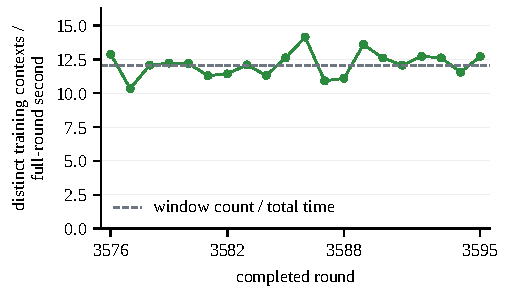
\includegraphics[width=\linewidth]{figures/fig_fw_live_round_throughput.pdf}
  \caption{\textbf{Completed-round throughput varies across rounds 3576--3595.}
  Twenty consecutive rounds, 3576--3595, captured at 09:54 UTC on
  2 November 2026. Each point divides \num{1219} distinct training contexts by
  that round's full wall time (contexts per second), including all work and
  waits. The dashed line divides the window's summed counts by summed time.
  Repeated contexts across rounds are not independent tasks; this is an
  operating observation, not \mbox{deployment} throughput.
  Scope: \cref{sec:method-status}.}
  \label{fig:fw-live-round-throughput}
  \end{minipage}\hfill
  \begin{minipage}[t]{\dimexpr.5\textwidth-.5\columnsep\relax}
  \vspace{0pt}
  \centering
  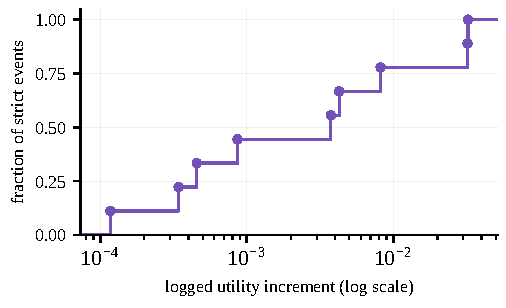
\includegraphics[width=\linewidth,height=2.05in,keepaspectratio]{figures/fig_fw_program_gain_distribution.pdf}
  \caption{\textbf{Nine strict program events occur across rounds 3656--3675.}
  Rounds 3656--3675, captured at 12:25 UTC on 2 November 2026.
  The empirical cumulative distribution gives each of the nine strict events
  equal weight; the horizontal axis is logarithmic. An increment is the
  journaled new utility minus its previous incumbent utility, computed
  from unrounded values. All 20 completed rounds are checked against the
  journal; 13 have no event and contribute no zero-gain observation.
  The window records zero adapter admissions. Event-level confidence
  intervals are unavailable; the curve is \mbox{descriptive,} without uncertainty
  bands. Scope: \cref{sec:method-status}.}
  \label{fig:fw-program-gain-distribution}
  \end{minipage}
  \par\medskip
  \begin{minipage}[t]{\dimexpr.5\textwidth-.5\columnsep\relax}
  \vspace{0pt}
  \centering
  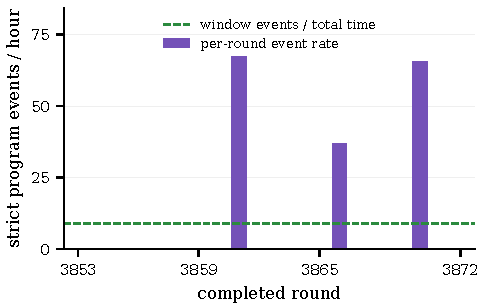
\includegraphics[width=\linewidth,height=2.05in,keepaspectratio]{figures/fig_fw_current_program_clock.pdf}
  \end{minipage}\hfill
  \begin{minipage}[t]{\dimexpr.5\textwidth-.5\columnsep\relax}
  \vspace{0pt}
  \caption{\textbf{Twelve strict program events occur across rounds 3931--3950.}
  Rounds 3931--3950, captured at 23:00 UTC on 2 November 2026.
  Bars divide each round's event count by its full wall time (events per hour);
  the dashed line divides the 12 events by the total
  \num{1987.27}\,s (21.74 events per hour). All 20 rounds are retained,
  including 10 with no event. The window records zero adapter admissions
  and no retained-utility gain; these program events do not measure
  independent first-proposal or game-day serving \mbox{performance. Scope: \cref{sec:method-status}.}}
  \label{fig:fw-current-program-clock}
  \end{minipage}
\end{figure*}

The 20-round 2696--2715 slice in \cref{fig:fw-round-throughput}, captured
at 06:54 UTC on 1 November 2026, has no adapter admission. Summary and
admission journals agree on candidate utility, recorded best, acceptance
and best-round identity. \Cref{fig:fw-live-round-throughput} adds a later
capture. Completed-round throughput divides distinct training contexts
by full round time; it differs from presentations per training second and
does not count \mbox{distinct tasks across} rounds.

The increments in \cref{fig:fw-program-gain-distribution} are logged
utility changes, not Elo changes or independent performance estimates.
The event counts in \cref{fig:fw-current-program-clock} are checked
against the promotion journal.
